\setcounter{figure}{1}
\begin{figure}[t!]
\centering
\setlength{\unitlength}{0.85\textwidth}%
\begin{picture}(1,0.8206)% original image aspect ratio
  \put(0,0){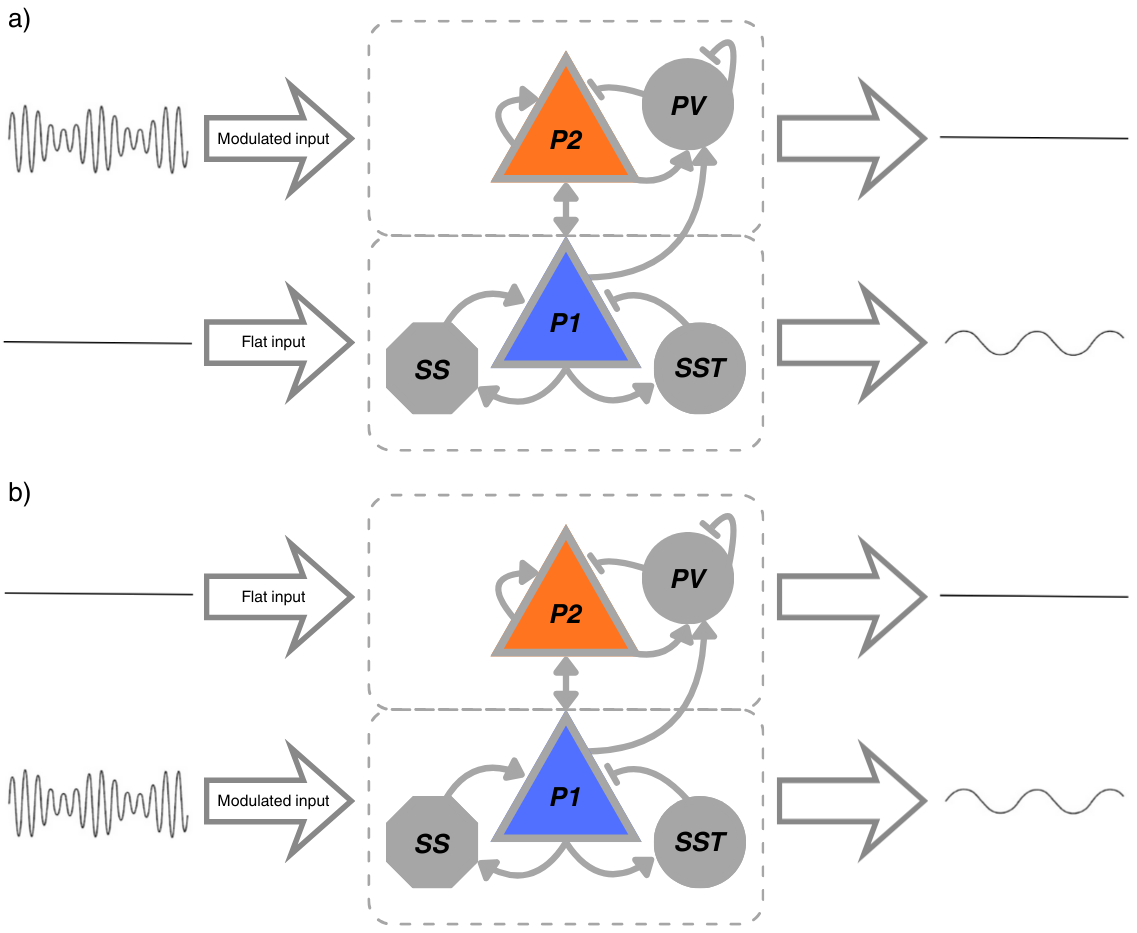
\includegraphics[width=\unitlength]{fig_lanmm_setup.png}}
  \put(0,0.788){\colorbox{white}{\makebox[0.045\unitlength][l]{\rule[-0.4ex]{0pt}{2.4ex}\textbf{(a)}}}}
  \put(0,0.371){\colorbox{white}{\makebox[0.045\unitlength][l]{\rule[-0.4ex]{0pt}{2.4ex}\textbf{(b)}}}}
\end{picture}
\caption{\textbf{Stimulation setup in a LaNMM column.} The column couples a
superficial PING subcircuit (pyramidal $P_2$ + PV; gamma) and a deep JR
subcircuit (pyramidal $P_1$ + SS + SST; alpha). \emph{(a)} the TI field drives
$P_2$ while $P_1$ receives a flat drive; \emph{(b)} the TI field drives $P_1$
while $P_2$ is flat. Through the sigmoid nonlinearities and $P_1$--$P_2$ coupling,
the generated beat-frequency component is transferred to the deep loop: $P_2$ carries the
modulated fast carrier, while $P_1$ exposes the recovered low-frequency component (right
traces).}
\label{fig:lanmm_setup}
\end{figure}
